\documentclass[10pt]{beamer}

% mac版,texShop 中Typeset选择 XeLaTex 

%%%%%%%%%%%%%%%%%%%%%%%%%%%%%%%%%%%%%
\usepackage[slantfont,boldfont]{xeCJK}
%\input{xecjkfonts},CJKtextspaces
\setCJKmainfont{STKaiti}   % STFangsong 设置缺省中文字体
\setCJKmonofont{SimSun}   % 设置等宽字体
\setmainfont{Times} % 英文衬线字体
\setmonofont{Times} % 英文等宽字体
\setsansfont{Times} % 英文无衬线字体
%%%%%%%%%%%%%%%%%%%%%%%%%%%%%%%%%%%%%%

\mode<presentation> {
  %\usetheme{Madrid}
  %\usetheme{Singapore}
  \usetheme{Warsaw}
  \setbeamercovered{transparent}
 % \usefonttheme[onlymath]{serif}  
 \usefonttheme{professionalfonts}%{structurebold}
 % \usefonttheme[onlymath]{structurebold}
  \usecolortheme{rose}
}

\usepackage[english]{babel}
%\usepackage[latin1]{inputenc}

%\usepackage{times}
%\usepackage[T1]{fontenc}


%\usepackage{epsfig}
\usepackage{graphics}
\usepackage{color}
\usepackage{amsmath,amssymb,mathrsfs}
\usepackage{amsfonts,stmaryrd}
%\usepackage{thmmarks}
%\usepackage{}



\newcommand\frakfamily{\usefont{U}{yfrak}{m}{n}}
\DeclareTextFontCommand{\textfrak}{\frakfamily}
\def\diag{\mathrm{diag}}


\title[数值计算方法]{数值计算方法}
\subtitle{-求解非线性方程}


\subject{Talks}

% If you have a file called "university-logo-filename.xxx", where xxx
% is a graphic format that can be processed by latex or pdflatex,
% resp., then you can add a logo as follows:

% \pgfdeclareimage[height=0.5cm]{university-logo}{university-logo-filename}
% \logo{\pgfuseimage{university-logo}}

%\pgfdeclareimage[height=0.5cm]{university-logo}{ncsu_logo}
%\logo{\pgfuseimage{university-logo}}

% Delete this, if you do not want the table of contents to pop up at
% the beginning of each subsection:
%\AtBeginSubsection[] {
%  \begin{frame}<beamer>
%    \frametitle{Outline}
%    \tableofcontents[currentsection,currentsubsection]
%  \end{frame}
%}

% If you wish to uncover everything in a step-wise fashion, uncomment
% the following command:

% \beamerdefaultoverlayspecification{<+->}


\setbeamertemplate{theorems}[numbered]
\setbeamertemplate{caption}[numbered]


\newtheorem{proposition}[theorem]{Proposition}

%%%%%%%%%%%%%%%%%%%%%%%%%%%
% REMARK-STYLE-ENVIRONMENTS %
%%%%%%%%%%%%%%%%%%%%%%%%%%%
\newcounter{remark}
% \numberwithin{theorem}{section}
\def\openrem#1#2{\refstepcounter{remark}\bigskip

{\noindent\bf#1~\theremark\if#2!{. }\else{ (#2).}\fi}
\it}
\def\thmskip{}
\newenvironment{remark}[1][!]{\openrem{Remark}{#1}}{\thmskip}

%%%%%%%%%%%%%%%%%%%%%%%%%%%%
%% AlGORITHM-STYLE-ENVIRONMENTS %
%%%%%%%%%%%%%%%%%%%%%%%%%%%%
\newcounter{algorithm}
% \numberwithin{theorem}{section}
\def\openalg#1#2{\refstepcounter{algorithm}\bigskip

{\noindent\bf#1~\thealgorithm\if#2!{. }\else{ (#2).}\fi}
\it}
\def\thmskip{}
\newenvironment{algorithm}[1][!]{\openrem{Algorithm}{#1}}{\thmskip}
%
%
%%%%%%%%%%%%%%%%%%%%%%%%%%%%
%% Result-STYLE-ENVIRONMENTS %
%%%%%%%%%%%%%%%%%%%%%%%%%%%%
%\newcounter{result}
%\def\openrem#1#2{\refstepcounter{result}\bigskip
%{\noindent \it \bfseries#1~\theremark\if#2!{. }\else{ (#2). }\fi}}
%\newenvironment{result}[1][!]{\openrem{Result}{#1}}{\qed}




%%%%%%%%%%%%%%%%%%%%%%%%%%%
%Redefine the Symbols%
%%%%%%%%%%%%%%%%%%%%%%%%%%%

\def\mathbi#1{\textbf{\em #1}}

% integrals
\def\dx{\,{\rm d}x}
\def\dxb{\,{\rm d}\boldsymbol{x}}
\def\dy{\,{\rm d}y}
\def\dt{\,{\rm d}t}
\def\ds{\,{\rm d}s}
\def\du{\,{\rm d}u}

\def\dr{\,{\rm d}r}
\def\dtheta{\,{\rm d}\theta}

\def\dd{{\rm d}}

\def\intOm{\int_{\Omega}}
\def\intbOm{\int_{\partial \Omega}}

% differences
\def\Dx{\Delta x}
\def\Dt{\Delta t}
\def\D{\Delta}


% operators
\def\Ls{\mathscr{L}}

% matirices
\def\Js{\mathscr{J}}


%fields%
\def\R{\mathbb{R}}
\def\N{\mathbb{N}}
\def\Z{\mathbb{Z}}

%Spaces%
\def\H{\mathbb{H}}
\def\L{\mathbb{L}}
\def\P{\mathbb{P}}


\def\U{\mathbb{U}}
\def\V{\mathbb{V}}
\def\W{\mathbb{W}}
\def\X{\mathbb{X}}
\def\Y{\mathbb{Y}}

\def\Cinfty{C^\infty}




%vectors%
\def\ab{\boldsymbol{a}}
\def\bb{\boldsymbol{b}}
\def\cb{\boldsymbol{c}}
\def\db{\boldsymbol{d}}
\def\eb{\boldsymbol{e}}
\def\fb{\boldsymbol{f}}
\def\gb{\boldsymbol{g}}
\def\hb{\boldsymbol{h}}
\def\nb{\boldsymbol{n}}
\def\rb{\boldsymbol{r}}
\def\sb{\boldsymbol{s}}


\def\ub{\boldsymbol{u}}
\def\vb{\boldsymbol{v}}
\def\wb{\boldsymbol{w}}
\def\xb{\boldsymbol{x}}
\def\yb{\boldsymbol{y}}
\def\zb{\boldsymbol{z}}

\def\Bb{\boldsymbol{B}}
\def\Cb{\boldsymbol{C}}
\def\Eb{\boldsymbol{E}}
\def\Fb{\boldsymbol{F}}
\def\Ib{\boldsymbol{I}}
\def\Kb{\boldsymbol{K}}
\def\Ob{\boldsymbol{O}}
\def\Qb{\boldsymbol{Q}}
\def\Rb{\boldsymbol{R}}
\def\Sb{\boldsymbol{S}}
\def\Ub{\boldsymbol{U}}
\def\Vb{\boldsymbol{V}}
\def\Wb{\boldsymbol{W}}
\def\Xb{\boldsymbol{X}}
\def\Yb{\boldsymbol{Y}}
\def\Zb{\boldsymbol{Z}}

%domains%
\def\Om{\Omega}
\def\bd{\partial}
\def\bOm{\bar{\Omega}}

%bold symbols%
\def\alphab{\boldsymbol{\alpha}}
\def\phib{\boldsymbol{\varphi}}

%energy%
\def\Jc{\mathcal{J}}
\def\Oc{\mathcal{O}}

%Greeks%
\def\vphi{\varphi}

%Special Functions%
\def\supp{\rm{supp}}
\def\sym{\rm{sym}}

\def\gradu{\nabla u}
\def\gradv{\nabla v}

%Mesh%
\def\Ts{\mathcal{T}}

\def\mach{\rm{mach}}


\begin{document}

\setbeamertemplate{itemize item}[triangle]

\begin{frame}
\titlepage
\end{frame}


\begin{frame}
  \frametitle{本节概要}
  \tableofcontents%[pausesections]
  % You might wish to add the option [pausesections]
%  \begin{itemize}
%  \item 显示Euler法及其误差分析
%  \item Taylor展开法
%  \item 
%  \end{itemize}
\end{frame}

\section{求解非线性方程概述}

\begin{frame}
\frametitle{求解非线性方程概述}
非线性科学是当今科学发展的一个重要方向,而求解非线性方程是现代科学中不可或缺的内容。我们通常利用数值方法求满足指定精度要求的近似解。\\

\begin{definition}[函数的根]
我们通常称函数$f(x)$在$x = r$处有根如果$f(r) = 0$。
\end{definition}

\begin{remark}
习惯上说,多项式的零点称为根,在求解非线性方程时,我们也把一般函数的零点称为根。
\end{remark}


\end{frame}






%%%%%%%%%%%%%%%%%%%%%%%%%%%%%%%%%%%%%%%%%%


\section{二分法}



\begin{frame}
\frametitle{确定有根区间}
解方程的第一步是确定有根的区间,这里我们可以利用连续函数的中值定理来寻找这个区间,具体来说我们有
\begin{theorem}
设$f$是$[a,b]$上的连续函数且满足$f(a)f(b) < 0$。则$f$在$[a,b]$上有根,即存在$r \in [a,b]$使得$f(r) = 0$。
\end{theorem}
定理可以直接利用连续函数中值定理证明,并可以由下图直观的表现。
\begin{figure}
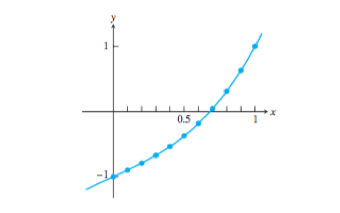
\includegraphics[width=4.5cm]{figs/Bracketing_Roots_1.png} 
\caption{$f(x) = x^3 + x -1$的图像} 
\end{figure}

\end{frame}

\begin{frame}
\frametitle{二分法}
虽然画图可以让我们大致观察到根所在的区间,但是一般我们并不能够用这样的方法来确定根所在的具体位置,一般来说我们利用二分法这种算法来寻找根。
\begin{algorithm}[二分法伪代码]\\
利用条件$f(a)f(b)$确定有根的区间$[a,b]$,确定精度$TOL$。\\
\rm{while} $\frac{(b-a)}{2} > TOL $ \\
\quad $c$ = $\frac{a+b}{2}$ \\
\quad \rm{if} $f(c) = 0$\\
\quad \quad 停机,结束程序输出$c$ \\
\quad \rm{if} $f(a)f(c) < 0$ \\
\quad \quad $b = c$ \\
\quad \rm{else} \\
\quad \quad $a = c$ \\
\quad \rm{end}\\
\rm{end} \\
最终的区间$[a,b]$必定含有根,并输出$\frac{a+b}{2}$作为根的近似。
\end{algorithm}
\end{frame}


\begin{frame}
\frametitle{二分法应用举例}
\begin{example}
在区间$[0,1]$上利用二分法寻找函数$f(x) = x^3 + x -1$的根。
\end{example}
我们注意到$f(0) f(1) = (-1)(1) < 0$,因此在$[0,1]$上必定有根。之后的计算可以用下表来表示并可以在Matlab中通过调节$TOL$的值将根所在的区间长度缩小。
\begin{figure}
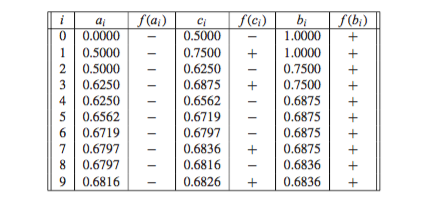
\includegraphics[width=7cm]{figs/bisection_method_example_1.png} 
\caption{利用二分法在$[0,1]$上寻找$f(x) = x^3 + x -1$的计算过程} 
\end{figure}
\end{frame}

\begin{frame}
\frametitle{二分法的误差}
如果$[a,b]$是初始的搜索区间,则$n$次二分之后,搜索区间缩小为了$\frac{b-a}{2^n}$,设$n$次二分后的区间为$[a_n,b_n]$,则$x_c = \frac{a_n+b_n}{2}$作为根$r$的近似。我们发现,由于搜索区间缩小为了$\frac{b-a}{2^n}$,所以误差有以下的上界
\begin{equation}
\text{解的误差} = |x_c - r| < \frac{b-a}{2^{n+1}}.
\end{equation}
同时,此时函数求值的次数为$n+2$次。

\begin{definition}
如果解的误差小于$0.5 \times 10^{-p}$,则我们称方程的解精确到小数点后$p$位。
\end{definition}

\end{frame}

\begin{frame}
\frametitle{二分法的误差}
\begin{example}
利用二分法寻找$f(x) = \cos x - x$在$[0,1]$上的根,并要求精确到小数点后六位。
\end{example}
由于在$n$次二分后,近似解的误差上界满足$\frac{b-a}{2^{n+1}} = \frac{1}{2^{n+1}}$,利用精确到小数点后$n$位的定义,我们有
\begin{figure}
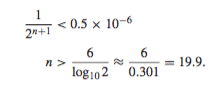
\includegraphics[width=4cm]{figs/bisection_method_example_2-1.png} 
\end{figure}
也就是说$20$步之后我们将会达到所要求的精度。
\end{frame}

\begin{frame}
\frametitle{二分法的误差}
计算过程可见下表
\begin{figure}
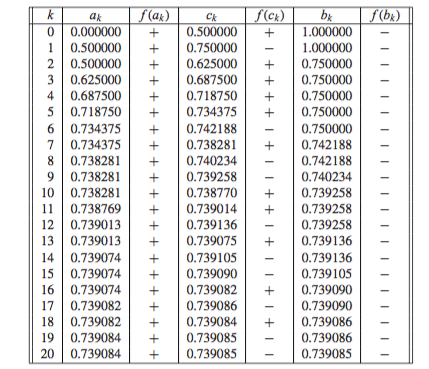
\includegraphics[width=5.5cm]{figs/bisection_method_example_2-2.png} 
\caption{二分法求$f(x) = \cos x -x$的根的计算过程}
\end{figure}
精确到六位小数的近似解为$0.739085$.
\end{frame}

\begin{frame}
\frametitle{等距离扫描法}
在确定有根区间时,如果函数比较简单,可以用画图的办法进行确定,但是如果函数比较复杂,那么进行一次求值需要的计算量比较大,而画图又需要大量的求值,那么画图法就不是一个好的方法。这里介绍一种等步长扫描法寻找有根的区间,具体算法如下。
\begin{algorithm}[等距离扫描法寻找有根区间]\\
$h>0$为给定步长,$b$为搜索上限,$h_m$为最小步长。\\
\rm{while} $h \ge h_m$ \\
取$x_0 = a, x_1 = a + h$。 \\
\quad \rm{while} $f(x_0) f(x_1)>0$ 且 $x_1 \le b$ \\
\quad \quad 令$x_0 = x_1$,$x_1 = x_1 +h$。\\
\quad \rm{end} \\
\quad \rm{if} $x_1<b$
\quad \quad 搜索成功输出$[x_0,x_1]$作为有根区间。\\
\quad \rm{else} \\
\quad \quad 令$h = \frac{h}{2}$。\\
\quad \rm{end} \\
\rm{end}
\end{algorithm}

\end{frame}


%%%%%%%%%%%%%%%%%%%%%%%%%%%%%%%%%%%%%%%%%%

\section{不动点迭代}

\begin{frame}
\frametitle{不动点}
\begin{definition}[不动点]
如果实数$r$满足$g(r) = r$,则$r$被称为函数$g(x)$不动点。
\end{definition}
例如$f(x) = \cos x - x$的根就是$g(x) = \cos x$的不动点,因为$g(x) = \cos x = x$等价于$f(x) = \cos x - x =0$。
\begin{definition}[不动点迭代]
当我们将$f(x) = 0$等价的写为$g(x) = x$后,不动点迭代就是将一个初始猜测$x_0$代入$g(x)$,并且对$g$进行迭代
\begin{equation}
x_{i+1} = g(x_i), i = 0,1,2,\ldots
\end{equation}
进而得到数列$\{x_i\}_{i = 0}^\infty$。
\end{definition}

\end{frame}

\begin{frame}
\frametitle{不动点迭代序列与不动点}
通过不动点迭代的得到的数列并不一定能保证收敛,但是根据上一章的连续极限定理,如果不动点迭代得到的序列是收敛的,则这个收敛的序列必定收敛于$g(x)$的不动点,这是因为
\begin{equation}
r = \lim_{i \rightarrow \infty} x_{i+1} = \lim_{i \rightarrow \infty} g(x_i) = g(  \lim_{i \rightarrow \infty} x_i) = g(r),
\end{equation}
其中第三个等号我们用到了连续收敛定理。
\vspace{0.5cm}

以上式子能够成立的前提是迭代序列收敛。对于寻找同一个函数$f(x)$的根,我们可以构造出很多不同的迭代函数$g(x)$,但并不是每一个迭代函数$g(x)$都会得到收敛序列。我们通过以下的例子来说明这一点。

\end{frame}

\begin{frame}
\frametitle{不动点迭代的收敛性}
\begin{example}
将求解$f(x) = x^3 + x -1 = 0$的问题换为不同的不动点迭代问题,并进行迭代。
\end{example}
我们选择以下几种方法将$f(x) = 0$转化为$g(x) = x$。

\begin{enumerate}
\item 第一种方法
\begin{equation}
\label{eq: FPI_Ex_1_g1}
g_1(x) = 1- x^3.
\end{equation}
\item 第二种方法
\begin{equation}
\label{eq: FPI_Ex_1_g2}
g_2(x) = (1-x)^{\frac{1}{3}}.
\end{equation}
\item 第三种方法
\begin{equation}
\label{eq: FPI_Ex_1_g3}
g_3(x) = \frac{1+2x^3}{1+3x^2}.
\end{equation}
\end{enumerate}

\end{frame}

\begin{frame}
\frametitle{不动点迭代的收敛性}
对于三个不同的迭代函数,如果选择初始猜测为$x_0 = 0.5$,则迭代的结果如下面几个表所示
\begin{figure}
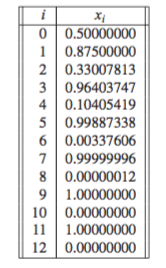
\includegraphics[width=3cm]{figs/FPI_g1_results.png} 
\caption{不动点迭代$g_1(x) = 1- x^3$的计算结果} 
\end{figure}

\end{frame}

\begin{frame}
\frametitle{不动点迭代的收敛性}
\begin{figure}
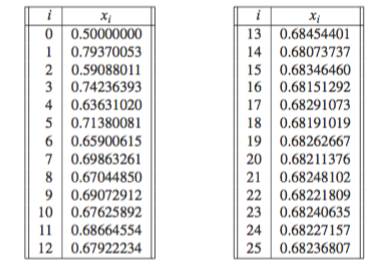
\includegraphics[width=6cm]{figs/FPI_g2_results.png} 
\caption{不动点迭代$g_2(x) = (1-x)^{\frac{1}{3}}$的计算结果} 
\end{figure}

\end{frame}

\begin{frame}
\frametitle{不动点迭代的收敛性}
\begin{figure}
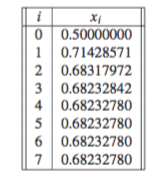
\includegraphics[width=3.5cm]{figs/FPI_g3_results.png} 
\caption{不动点迭代$g_3(x) =  \frac{1+2x^3}{1+3x^2}$的计算结果} 
\end{figure}

可以看到,迭代函数$g_1$无法生成收敛的序列,迭代函数$g_2$通过$20$步左右的迭代值稳定在$0.682$附近,而迭代函数$g_3$则通过$4$次迭代就将迭代序列的值稳定在了$0.68232780$,即小数点后$8$位。可以看到迭代函数选取不同迭代效果差别非常大。
\end{frame}


\begin{frame}
\frametitle{不动点迭代的几何解释}
以上几个不动点迭代的结果可以用以下图片更直观的解释。
\begin{figure}
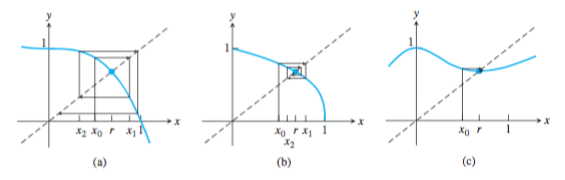
\includegraphics[width=12cm]{figs/FPI_geometry_1.png} 
\caption{不动点迭代的几何意义,(a)对应$g_1$,(b)对应$g_2$,(c)对应$g_3$} 
\end{figure}
\end{frame}

\begin{frame}
\frametitle{不动点迭代的线性收敛性}
不动点迭代的收敛性可以由两个线性函数的不动点迭代更清楚的表现出来。我们设
\begin{equation}
g_1(x) = -\frac{3}{2} x + \frac{5}{2}, \quad g_2(x) = -\frac{1}{2}x + \frac{3}{2}.
\end{equation}
容易得到,$x = 1$是这两个函数的不动点。但是下图可以看到两个不动点迭代的区别。
\begin{figure}
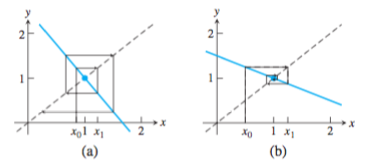
\includegraphics[width=7.5cm]{figs/FPI_geometry_2.png} 
\caption{不动点迭代的几何解释,(a)对应$g_1$,(b)对应$g_2$} 
\end{figure}
\end{frame}


\begin{frame}
\frametitle{不动点迭代的线性收敛性}
事实上,两个迭代函数最大的区别是函数的斜率,即$g'(x)$的值。从方程的角度看,$r=1$是两个函数的不动点,对$g_1$,我们有
\begin{align}
g_1(x) = -\frac{3}{2}(x-1) +1, \nonumber \\
g_1(x)-1 = -\frac{3}{2}(x-1), \nonumber \\
x^1_{i+1} -1 = -\frac{3}{2}(x^1_i-1).
\end{align}
对$g_2$,我们有
\begin{align}
g_2(x) = -\frac{1}{2}(x-1) +1, \nonumber \\
g_2(x)-1 = -\frac{1}{2}(x-1), \nonumber \\
x^2_{i+1} -1 = -\frac{1}{2}(x^2_i-1).
\end{align}
\end{frame}


\begin{frame}
\frametitle{不动点迭代的线性收敛性}
这里我们可以看出,如果令$e^1_i = |x^1_i -1|$为$g_1$迭代到第$i$步后的误差绝对值,$e^2_i = |x^2_i -1|$为$g_2$迭代到第$i$步后的误差的绝对值,我们可以发现$e^1_{i+1} = \frac{3}{2} e^1_i$,而$e^2_{i+1} = \frac{1}{2} e^2_i$,即迭代函数$g_1$产生的误差不断扩大,而迭代函数$g_2$产生的误差不断缩小。为了更一般的讨论不动点迭代的收敛性,我们有如下定义。

\begin{definition}[线性收敛]
令$e_i$表示一个迭代方法在第$i$步迭代后的误差的绝对值。如果
\begin{equation}
\lim_{i \rightarrow \infty} \frac{e_{i+1}}{e_i} = S <1,
\end{equation}
则称这个方法具有线性收敛性,且收敛率为$S$。
\end{definition}
\end{frame}

\begin{frame}
\frametitle{不动点迭代的线性收敛性}
\begin{definition}[局部收敛]
对于一个迭代方法,如果初始猜测$x_0$足够靠近$r$就能够产生收敛于$r$的迭代序列,则称这个迭代法是局部收敛的。
\end{definition}

根据这些定义,我们有如下定理
\begin{theorem}[不动点迭代的线性收敛性]
假设$g$是一个连续可导函数满足$g(r) = r$且$S = |g'(r)| < 1$。则当初始猜测$x_0$足够靠近不动点$r$时,由$g$这个函数定义的不动点迭代所产生的迭代序列收敛于不动点$r$,且这个收敛是线性的,收敛率为$S$。
\end{theorem}
\end{frame}


\begin{frame}
\frametitle{不动点迭代应用举例}
\begin{example}
利用不动点迭代寻找$\cos x = \sin x$的根。
\end{example}
我们将这个问题转化为求$g(x) = x + \cos x - \sin x$的不动点的问题。求解的结果可以由下表表示
\end{frame}


\begin{frame}
\frametitle{不动点迭代应用举例}
\begin{figure}
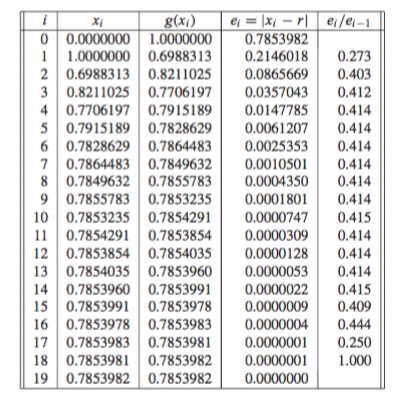
\includegraphics[width=6.5cm]{figs/FPI_Ex_1_Results.png} 
\caption{$g(x) = x + \cos x - \sin x$的迭代结果} 
\end{figure}
\end{frame}

\begin{frame}
\frametitle{不动点迭代应用举例}
在这个例子中我们可以观察到以下几点。
\begin{itemize}
\item 首先,迭代序列收敛到$0.7853982 \approx \frac{\pi}{4}$,因为$\cos  \frac{\pi}{4} = \sin  \frac{\pi}{4}$。
\item 第二,表的第四列列出了迭代序列与真解$\frac{\pi}{4}$之间的误差,这个误差随着迭代的进行逐步减小。
\item 第三,表的第五列展示出了两步之间的误差的比值,可以看到,在大部分的时候这个比值停留在$0.414$。这与我们的理论推导是高度一致的,因为
\begin{equation}
S = |g'(r)| = |1 - \sin r - \cos r| = \Big|1- \frac{\sqrt{2}}{2} - \frac{\sqrt{2}}{2} \Big| = |1- \sqrt{2}| \approx 0.414.
\end{equation}
\end{itemize}
\end{frame}

\begin{frame}
\frametitle{停机准则}
与二分法不同,不动点迭代一般不能在计算开始之前确定迭代的步数,因为不动点迭代误差上界与迭代步数之间不存在如二分法一样的确定的公式。因此,我们需要用计算结果来确定是否停止迭代。一般的,迭代停止的准则(又称为停机准则)为
\begin{equation}
|x_{i+1} - x_i| < \rm{TOL},
\end{equation}
或者当解不接近于$0$时,停机准则为
\begin{equation}
\frac{|x_{i+1} - x_i|}{|x_{i+1}|} < \rm{TOL},
\end{equation}
其中TOL是预先设定的一个误差容许值。
当然,设$\theta>0$是一个接近于$0$的数,当解也接近于$0$的时候,我们可以用如下的混合停机准则
\begin{equation}
\frac{|x_{i+1} - x_i|}{\max\{|x_{i+1}|,\theta\}} < \rm{TOL}.
\end{equation}


\end{frame}




%%%%%%%%%%%%%%%%%%%%%%%%%%%%%%%%%%%%%%%%%%

\section{牛顿迭代}

\begin{frame}
\frametitle{牛顿迭代的几何意义}
牛顿迭代是一种特殊的不动点迭代,一般具有比二分法和大多数不动点迭代都快的收敛速度。牛顿迭代可以由以下的图像给出几何解释
\begin{figure}
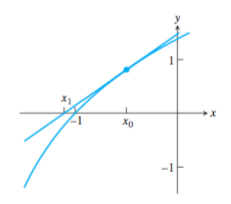
\includegraphics[width=5cm]{figs/Newton_geometry_1.png} 
\caption{牛顿迭代的几何解释} 
\end{figure}
\end{frame}


\begin{frame}
\frametitle{牛顿迭代的代数导出}
牛顿迭代还可以从代数的角度导出。我们将$f(r)$($f$在根$r$处的值)在根$x_0$处作Taylor展开
\begin{equation}
f(r) = f(x_0) + f'(x_0)(r-x_0) + \frac{f''(x_0)}{2!}(r-x_0)^2 + \ldots.
\end{equation}
取线性部分作为$f(r)$的近似
\begin{equation}
f(x_0) + f'(x_0)(r-x_0) \approx f(r) =0.
\end{equation}
若$f'(x_0) \neq 0$,则有
\begin{equation}
r \approx x_0 - \frac{f(x_0)}{f'(x_0)}.
\end{equation}
\end{frame}


\begin{frame}
\frametitle{牛顿迭代法}
根据以上的推导,我们可以构造牛顿迭代算法
\begin{algorithm}[牛顿迭代法] \\
$x_0 =$初始猜测 \\
$x_{i+1} = x_i - \frac{f(x_i)}{f'(x_i)}, i = 0, 1,2, \ldots$.
\end{algorithm}

\begin{example}
利用牛顿法解方程$x^3 + x -1 = 0$。
\end{example}
求导可得$f'(x) = 3x^2 + 1$,则由牛顿迭代得
\begin{align}
x_{i+1} & = x_i - \frac{x_i^3 + x_i - 1}{3x_i^2 + 1} \nonumber \\
            & = \frac{2x_i^3 + 1}{3x_i^2 + 1}.
\end{align}
\end{frame}


\begin{frame}
\frametitle{牛顿迭代法}
计算结果见下表
\begin{figure}
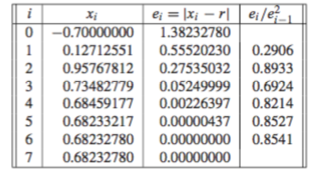
\includegraphics[width=6.5 cm]{figs/Newton_Ex_1_Results.png} 
%\caption{$g(x) = x + \cos x - \sin x$的迭代结果} 
\end{figure}
\end{frame}


\begin{frame}
\frametitle{牛顿迭代法}
迭代的图示如下
\begin{figure}
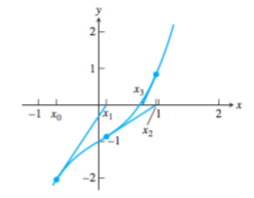
\includegraphics[width=6 cm]{figs/Newton_Ex_1_Figure.png} 
\caption{$f(x) = x^3 + x -1 = 0$牛顿迭代示意图} 
\end{figure}
\end{frame}


\begin{frame}
\frametitle{牛顿迭代法的二阶收敛性}
\begin{definition}
令$e_i$表示第$i$步的迭代结果,如果某种迭代法误差的绝对值满足
\begin{equation}
M = \lim_{i \rightarrow \infty} \frac{e_{i+1}}{e_i^2} < \infty,
\end{equation}
则称这种迭代法是二阶收敛的。
\end{definition}

\begin{theorem}[牛顿迭代的二阶收敛性]
\label{thm: quadratic convergence Newton}
假设$f$是二阶连续可导函数且$f(r)=0$。如果$f'(r) \neq 0$,则牛顿迭代局部且二阶收敛到$r$。第$i$步迭代结果的误差的绝对值$e_i$满足
\begin{equation}
\lim_{i \rightarrow \infty} \frac{e_{i+1}}{e_i^2} = M = \frac{f''(r)}{2f'(r)}.
\end{equation}
\end{theorem}
\end{frame}


\begin{frame}
\frametitle{线性收敛和二阶收敛性的比较}
设$S = |g'(r)|$,其中$g$为不动点迭代函数,$r$为不动点,我们有
\begin{equation}
e_{i+1} \approx S e_i,
\end{equation}
而牛顿迭代的有
\begin{equation}
e_{i+1} \approx M e_i^2.
\end{equation}
我们可以发现
\begin{enumerate}
\item 当$e_i<1$开始,二阶收敛的速度明显较线性收敛快。
\item $S$的值对于线性收敛非常重要,因为只有$S<1$时,迭代才可能收敛。
\item $M$的值对于二阶收敛并不重要,因为只要$M$不是很大,$e_i^2$会很快占主导。
\end{enumerate}
\end{frame}


\begin{frame}
\frametitle{牛顿迭代的线性收敛性}
定理\ref{thm: quadratic convergence Newton}并不意味着对于任意的$f(x) = 0$的求根问题都是二阶收敛。
\begin{example}
利用牛顿迭代寻找$f(x) = x^2$的根。
\end{example}
利用牛顿迭代
\begin{align}
x_{i+1} & = x_i - \frac{f(x_i)}{f'(x_i)} \nonumber \\
            & = x_i - \frac{x_i^2}{2x_i} \nonumber \\
            & = \frac{x_i}{2}.
\end{align}
\end{frame}


\begin{frame}
\frametitle{牛顿迭代的线性收敛性}
以下是这样的计算结果
\begin{figure}
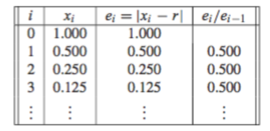
\includegraphics[width=6 cm]{figs/Newton_Ex_2_Results.png} 
\caption{$f(x) = x^2$牛顿迭代示意图} 
\end{figure}
\end{frame}


\begin{frame}
\frametitle{牛顿迭代的线性收敛性}
\begin{example}
利用牛顿迭代寻找$f(x) = x^m$的根。
\end{example}
利用牛顿迭代
\begin{align}
x_{i+1} & = x_i - \frac{x_i^m}{m(x_i^{m-1})} \nonumber \\
            & = \frac{m-1}{m} x_i.
\end{align}
因为$r = 0$,令$e_i = |x_i - r| = x_i$,有
\begin{equation}
e_{i+1} = S e_i = \frac{m-1}{m} e_i.
\end{equation}
\end{frame}

\begin{frame}
\frametitle{牛顿迭代的线性收敛性}
\begin{theorem}
设$f$在$[a,b]$上是$(m+1)-$阶连续可导函数,且在$r \in [a,b]$处有$m$重根。则牛顿法局部收敛到$r$,而第$i$步的误差的绝对值$e_i$满足
\begin{equation}
\lim_{i \rightarrow \infty} \frac{e_{i+1}}{e_i} = S,
\end{equation}
其中
\begin{equation}
S = \frac{m-1}{m}.
\end{equation}
\end{theorem}

造成牛顿迭代线性收敛的原因是,在重根$r$处,$f'(r) = 0$,与牛顿迭代二阶收敛的条件$f'(r)\neq 0$相矛盾。
\end{frame}


\begin{frame}
\frametitle{改进的牛顿迭代}
如果某个根的重数$m$在事先是知道的,那么可以通过改进得到二阶收敛的牛顿迭代。

\begin{theorem}[改进的牛顿迭代的二阶收敛性]
设$f$在$[a,b]$上是$(m+1)-$阶连续可导函数,且在$r \in [a,b]$处有$m$重根,则改进的牛顿迭代\begin{equation}
x_{i+1} = x_i - \frac{m f(x_i)}{f'(x_i)}
\end{equation}
局部二阶收敛到根$r$。
\end{theorem}
\end{frame}


\begin{frame}
\frametitle{改进的牛顿迭代}
\begin{example}
通过数值方法寻找$f(x) = \sin x + x^2 \cos x - x^2 -x$的根$r = 0$。
\end{example}
对$f(x)$求导,我们发现
\begin{align}
f'(x) = \cos x + 2x \cos x - x^2 \sin x - 2x -1, \nonumber \\
f''(x) = -\sin x + 2 \cos x - 4x \sin x - x^2 \cos x -2, \nonumber \\
f'''(x) = -\cos x - 6 \sin x - 6x \cos x + x^2 \sin x.
\end{align}
由此得$f(0) = f'(0) = f''(0) =0$而$f'''(0) = -1$。.构造牛顿迭代
\begin{align}
x_{i+1} & = x_i - \frac{f(x_i)}{f'(x_i)} \nonumber \\
            & = x_i - \frac{\sin x_i + x_i^2 \cos x_i - x_i^2 -x_i}{-\sin x_i + 2 \cos x_i - 4x_i \sin x_i - x_i^2 \cos x_i -2}.
\end{align}
\end{frame}

\begin{frame}
\frametitle{改进的牛顿迭代}
计算结果如下表,可以观察到$\frac{e_{i+1}}{e_{i}} \approx \frac{2}{3}$。
\begin{figure}
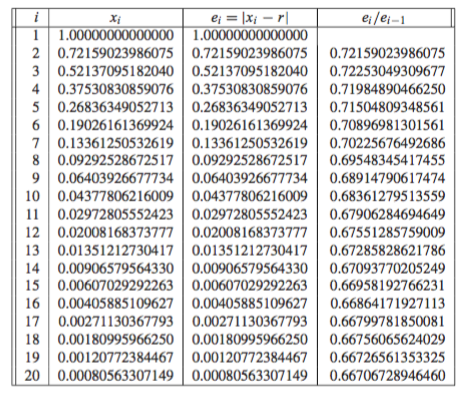
\includegraphics[width=6 cm]{figs/Newton_Ex_3_Results-1.png} 
\caption{利用牛顿迭代计算$f(x) = \sin x + x^2 \cos x - x^2 -x$根的结果} 
\end{figure}
\end{frame}

\begin{frame}
\frametitle{改进的牛顿迭代}
如果构造改进的牛顿迭代
\begin{align}
x_{i+1} & = x_i - \frac{3f(x_i)}{f'(x_i)} \nonumber \\
            & = x_i - \frac{3(\sin x_i + x_i^2 \cos x_i - x_i^2 -x_i)}{-\sin x_i + 2 \cos x_i - 4x_i \sin x_i - x_i^2 \cos x_i -2},
\end{align}
则计算结果如下
\begin{figure}
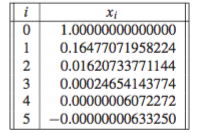
\includegraphics[width=3.5 cm]{figs/Newton_Ex_3_Results-2.png} 
\caption{利用改进的牛顿迭代计算$f(x) = \sin x + x^2 \cos x - x^2 -x$根的结果} 
\end{figure}
\end{frame}


\begin{frame}
\frametitle{牛顿迭代小结}
牛顿迭代是非常重要的求解非线性方程根的方法,最大的优点是收敛速度快,尤其是当迭代值落入局部收敛区域的时候,往往几步迭代就可以得到比较精确的解。

\vspace{0.2cm}
但牛顿迭代不是万能的,如果初值选区不当很可能会出现牛顿迭代发散的情况产生,并且在迭代结果为重根的时候只有线性的收敛速度。除此之外,牛顿迭代需要计算一阶导数,在导数比较复杂的时候,会产生较大的计算量。

\end{frame}



%%%%%%%%%%%%%%%%%%%%%%%%%%%%%%%%%%%%%%%%%%
\section{无导数求解非线性方程}

\begin{frame}
\frametitle{无导数求解非线性方程}
牛顿迭代的其中一个缺点是需要求函数的一阶导数,这在导数比较复杂的时候会产生较大的计算量,甚至是不可能求出来的,因此,我们需要用一些其它方法代替牛顿迭代。这里介绍几个牛顿迭代常用的变形。
\end{frame}

\begin{frame}
\frametitle{割线法}
割线法与牛顿迭代类似,主要区别是利用一个差分来代替导数,从几何上说,就是将切线用一条割线代替。具体来说,在已知前两次迭代结果$x_i$和$x_{i-1}$的时候,我们利用
\begin{equation}
f'(x_i) \approx \frac{f(x_i) - f(x_{i-1})}{x_i-x_{i-1}},
\end{equation}
得到割线法:
\begin{algorithm}[割线法]\\
$x_0, x_1$为初始猜测 \\
$x_{i+1} = x_i - \frac{f(x_i)(x_i-x_{i-1})}{f(x_i) - f(x_{i-1})}, i = 1,2,3, \ldots$
\end{algorithm}
\end{frame}



\begin{frame}
\frametitle{割线法的超线性收敛}
与不动点迭代和牛顿迭代不同,割线法需要两个初始值的猜测。

可以证明当割线法的迭代结果收敛到$r$且$f'(r) \neq 0$的时候,误差满足
\begin{equation}
e_{i+1} \approx \big|\frac{f''(r)}{2f'(r)}\big| e_i e_{i-1},
\end{equation}
进而可以证明
\begin{equation}
e_{i+1} \approx \big|\frac{f''(r)}{2f'(r)}\big|^{\alpha -1} e_i^{\alpha},
\end{equation}
其中$\alpha = \frac{1+\sqrt{5}}{2} \approx 1.62$。很明显,割线法的收敛比线性收敛好但比二阶收敛差一些,这样的收敛性一般称为超线性收敛。
\end{frame}


\begin{frame}
\frametitle{错位法}
错位法是割线法的另一个变形。假设我们知道函数的根在$[a,b]$中且$f(a)f(b) < 0$,那么令下一次的迭代结果为
\begin{equation}
c = a - \frac{f(a)(a-b)}{f(a) - f(b)} = \frac{bf(a) - af(b)}{f(a) - f(b)}.
\end{equation}
可以证明,因为$f(a)$与$f(b)$反号,所以$a \le c \le b$。接下来根据$f(a)f(c) < 0$或者$f(c)f(b) <0$来确定新的搜索区间。错位法的算法如下。
\end{frame}


\begin{frame}
\frametitle{错位法的算法}
\begin{algorithm}[错位法]\\
给出有根区间$[a,b]$且$f(a)f(b)<0$。\\
\rm{for} $i = 1,2,3, \ldots$\\
\quad $c = \frac{bf(a) - af(b)}{f(a) - f(b)}$\\
\quad \rm{if} $f(c)=0$,停机,输出$c$\\
\quad \rm{if} $f(a)f(c) <0$\\
\quad \quad $b=c$ \\
\quad \rm{else} \\
\quad \quad $a = c$\\ 
\quad \rm{end} \\
\rm{end}
\end{algorithm}
\end{frame}


\begin{frame}
\frametitle{课后阅读}
[NA] 第1章 1.1,1.2,1.4,1.5.1


\end{frame}

\end{document}

